\section{Algebra}
\label{sec:algebra}
\setlength{\textfloatsep}{5pt}% Remove \textfloatsep

In this section we describe the operators of \tg algebra.  The algebra
is compositional: all operators take a \tg or a pair of \tgs as input,
and produce a \tg.  Our algebra is based on the principles of snapshot
reducibility, which states that an operation should yield the same
result when applied to the temporal representation as it would if it
non-temporal version was applied separately to every snapshot state of
the temporal representation, and extended snapshot reducibility, which
requires that references to time can be used in the
operations~\cite{Dignos2012}.

%\subsection{Preliminaries}
%\label{sec:algebra:prelim}

\subsection{Maintaining integrity}
\label{sec:algebra:integrity}

Our algebra operates on \tgs, and so\eat{, in addition to keeping the
  data structure (and its constituent parts) coalesced,} we must
ensure that the result is a valid \tg.  One of the requirements of our
model is that each entity exists only once during any time instant
$t$.  To maintain this validity we introduce a {\em resolve} function.

\begin{definition}[Resolve function]
\eat{Let $((a_1,p_1),$ \\ $\ldots, (a_n,p_n))$ be a list of possible
  values of an attribute of a node or an edge along with their
  associated periods of validity.  A {\em resolve function} produces a
  single attribute value $a = resolve((a_1,p_1), \ldots, (a_n,p_n))$.}
Let $((a_l,p_l),(a_r,p_r))$ be a tuple of possible values of an
attribute of a node or an edge along with the associated validity
periods.  A {\em resolve function} produces a single attribute value
$a = resolve((a_l,p_l), (a_r,p_r))$.
\end{definition}

A resolve function can pick an arbitrary element, compute an average
for each property, put the values in a set, etc.  When applied over a
bag of values in a reduce fashion, a resolve function is an {\em
  aggregation function}.  We support the standard \{ \insql{count} |
\insql{min} | \insql{max} | \insql{sum} \}, which have their customary
meaning.  We also support \{ \insql{any} | \insql{first} |
\insql{last} | \insql{set} | \insql{bag} \}, which are possible to
compute because properties being resolved have temporal information.
\insql{first} and \insql{last} refer to the value of an attribute with
the earliest/latest timestamp, while \insql{set} and \insql{bag}
associate a key an unordered collection of values with the set or bag
semantics (but do not keep the associated validity periods).  Finally,
we support \{ \insql{left} | \insql{right} \}, which select the
attribute of the left, resp. right, operand.  Other, more complex,
functions can be defined by the user.

\begin{lemma}
Let $\psi$ be an n-ary temporal operator on \tg.  If $\psi^T (\ttt)$
produces multiple possible attribute values for any entity at the same
time instant, it must also specify a resolve function to compute a
single valid attribute value.
\end{lemma}

\eat{ This objective informed our design of
  the algebra, e.g., we did not include some flavors of temporal
  aggregation because the result would be invalid.  Further, this
  objective informs the rewriting of applicable operations over the
  \ve representation.}  

Each operator in our algebra produces a valid \tg.  We note which
operators are known to uncoalesce the output, thus requiring
coalescing, require FK enforcement, or include the resolve function.

\subsection{Unary operators}
\label{sec:algebra:unary}

We introduce three basic unary operators: slice, subgraph, and map.
%\subsection{Slice}
%\label{sec:algebra:slice}

{\bf Slice.}  The unary {\em slice} operator, denoted $\tau_c (\ttt)$,
where $c$ is a time period, cuts a temporal slice from \ttt.  The
resulting \tg will contain nodes and edges whose period $p$ has a
non-empty intersection with $c$.  To evaluate $\tau_c (\tve)$, we
apply $\tau_c$ to each of the four constituent relations of \tve:
$\tau_c (\tv) = \{ (v, p \cap c)~~|~~(v, p) \in \tv \wedge
(\pred{c}{overlaps}{p} \vee \pred{c}{contains}{p}) \}$, and
analogously for each \te, \tav and \tae.

\eat{If $p.start < c.start$ or $p.end > c.end$ for some tuple $(g,
  p)$, then $p$ is trimmed to be within the boundaries of $c$: $\tau_c
  (\trg) = \{ (g, p \cap c)~~|~~(g, p) \in \trg \wedge
  (\pred{c}{overlaps}{p} \vee \pred{c}{contains}{p})\}$.  }

Slice does not uncoalesce and does not require FK enforcement.  The
proofs for this and similar statements below are included in
Appendix~\ref{sec:app1}.

%\subsection{Temporal subgraph matching}
%\label{sec:algebra:subgraph}

{\bf Subgraph.}  Temporal subgraph matching is defined analogously to
subgraph matching in non-temporal graphs: it applies a predicate to
each node and edge of \tg. \eat{subgraph function $f$ to every
  representative graph of the input.  To ensure that a valid \tg is
  computed as a result of this operation, we restrict our attention to
  functions that compute a single subgraph of a given representative
  graph as a result: $\sigma_f (\trg) = \{ (g', p)~~|~~(g, p) \in \trg
  \wedge g' = f(g) \wedge$\\$V_{g'} \subseteq V_{g} \wedge E_{g'}
  \subseteq E_{g} \}$.}  Even more specifically, we focus on functions
that can be expressed as a pair of {\em conjunctive queries}
$\sigma_{C_V,C_E} (\ttt)$, where $C_V$ specifies predicates over the
vertices, and $C_E$ --- over the edges.  The predicates can be over
the attributes and also over the timestamps of the nodes/edges, to
support the extended snapshot reducibility.  Computing arbitrary
subgraphs of an evolving graph is beyond the scope of this paper, and
we defer this to future work.

$\sigma_{C_V,C_E} (\tve) = (\tv',\te',\tav',\tae') ~|~$ \\
$\tv' = \pi_{v,p} (\sigma_{C_{V1}} (\tv) \bowtie^T \sigma_{C_{V2}} (\tav)) \wedge \tav' = \sigma_{C_{V2}} (\tav)$ \\
$\te' = \pi_{v_1,v_2,p} (\sigma_{C_{E1}} (\te) \bowtie^T \sigma_{C_{E2}} (\tae)) \wedge \tae' = \sigma_{C_{E2}} (\tae)$.

\eat{Like other unary operators, $\sigma_{C_V, C_E} (\tve)$ follows the
outline of Algorithm~\ref{alg:op}.  Since $C_V$ and $C_E$ may involve
predicates over the attributes, we compute the join of the vertex
(resp. edge) relation with the corresponding attribute relation and
push selections:$\tv' = \pi_{v,p} (\sigma_{C_{V1}} (V) \bowtie
\sigma_{C_{V2}} (\tav))$ (line 1),$\te' = \pi_{v_1,v_2,p}
(\sigma_{C_{E1}} (E) \bowtie \sigma_{C_{E2}} (\tae))$ (line 2), $\tav'
= \sigma_{C_{V2}} (\tav)$ (line 3), $\tae' = \sigma_{C_{V2}} (\tae)$
(line 4).}

Subgraph does not uncoalesce, but does require FK enforcement for \tve.

%\subsection{Temporal map}
%\label{sec:algebra:project}

{\bf Map.}  The map operation applies user-defined map functions $M_V$
and $M_E$ to the vertices and edges of \tg.  To evaluate
$\map_{M_V,M_E} (\tve)$, we set $\tv'=\tv$ and $\te'=\te$, and compute
$\tav' = \map_{M_V}(\tav)$ and $\tae' = \map_{M_E}(\tae)$.

\eat{Temporal map iterates over the tuples of \trg, and applies the
user-specified map functions $M_V$ and $M_E$ to the vertices and edges
of each $g$: $\map_{M_V,M_E} (\trg) = \{(g', p)~~|~~(g,p) \in \trg
\wedge g'= \map_{M_V,M_E}(g)\}$.
}  

While map is an arbitrary user-specified function, there are some
common use cases.  Map can be used to remove vertex and edge
properties, as in projection.  In such cases we will use short-hand
notation similar to projection, listing the properties that we wish to
retain. For example, $\map_{M_V:{school},M_E:\emptyset} (\insql{T1})$
will keep only the school property of the vertices, and no properties
of the edges.  Another useful map operation eliminates duplicates in
the bag of a particular vertex or edge property.  \eat{It may also be
useful to flatten nested bags or aggregate multiple values of the same
property of a vertex or edge, e.g., compute a sum or an average
following temporal intersection or union
(Section~\ref{sec:algebra:join}).}

Map may uncoalesce \tav and \tae, but does not require FK enforcement.

\subsection{Binary operators}
\label{sec:algebra:binary}

We support the temporal versions of the three binary set operators
intersection ($\cap^T$), union ($\cup^T$), and difference
($\setminus^T$).  As Dignos et al. showed, these three operators are
not schema robust~\cite{Dignos2012}.  Schema robust operators are not
affected if the argument relation is extended by an additional
attribute.  This presents a problem when executing the set operations
over the \tav and \tae relations as there is no guarantee that a node
or an edge with the same identity and at the same time instant has the
same attribute set.  Thus all three operators require resolve
functions.

\begin{definition}[Set-theoretic operators]
Let $\oplus$ be a temporal set operator $\in \{ \cap^T, \cup^T,
\setminus^T \}$ and $r$ be a resolve function.  Then $\tve_1 \oplus_r
\tve_2 = \{ \tv_1 \oplus \tv_2, \te_1 \oplus \te_2, map_r(\tav_1
\fullouterjoin^T \tav_2),$\\ $map_r(\tae_1 \fullouterjoin^T \tae_2)
\}$, with all FK constraints on \tav and \tae enforced.
\end{definition}

Because the graphs do not have a fixed schema, it may not be desirable
to specify a resolve function for every possible property.  A default
resolve function is \insql{set}.

%\subsection{Temporal graph intersection}
%\label{sec:algebra:join}
\eat{
The binary temporal graph intersection operation $\trga \cap \trgb$
computes a temporal join~\cite{Gao2005} of \trga and \trgb with the
predicate $\trga.p \cap \trgb.p \neq \emptyset$, producing a tuple for
each pair of representative graphs for which time periods intersect:
$\trga \cap \trgb = \{(g_1 \cap g_2, p_1 \cap p_2)~|~((g_1, p_1) \in
\trga \wedge (g_2, p_2) \in \trgb \wedge p_1 \cap p_2 \neq \emptyset
\}$.  The result of $g_1 \cap g_2$ is computed by intersecting the
sets of vertices and of edges of the graphs~\cite{GraphTheory}.  For
each vertex and edge in the result, we compute a {\em union} of their
bags of properties.% \julia{Figure with example.}
%
Algorithm~\ref{alg:inter} presents the evaluation of $\tvea \cap
\tveb$. We compute temporal joins over \tv and \te (lines 1, 2).  We
then compute \tav' and \tae' with temporal outer joins of the
corresponding relations (lines 3, 4).  Finally, we enforce foreign key
constraints on \te', \tav' and \tae' (lines 5, 6).
}

%\begin{algorithm}[b]
%\caption{Temporal graph intersection in \tve.}
%\begin{algorithmic}[1]
%%\REQUIRE $\tvea (\tv_1;\te_1;\tav_1;\tae_1), \tveb (\tv_2;\te_2;\tav_2;\tae_2)$.\\
%\REQUIRE $\tvea, \tveb$.\\
%\STATE $\tv' = \tv_1 \Join^T_v \tv_2$\\ 
%\STATE $\te' = \te_1 \Join^T_{v_1,v_2} \te_2$\\ 
%\STATE $\tav' = \cl (\pi_{v,p,\tav_1.a \cup \tav_2.a}\tav_1 \fullouterjoin^T_v \tav_2)$\\
%\STATE $\tae' = \cl (\pi_{v_1,v_2,p,\tae_1.a \cup \tae_2.a}\tae_1 \fullouterjoin^T_{v_1,v_2} \tae_2)$\\
%\STATE $\tae' = \pi_{a_1 \cap a_2}(\tae_1 \Join^T \tae_2)$\\
%\STATE enforce foreign keys on $\tav'$ w.r.t. $\tv'$\\ 
%\STATE enforce foreign keys on $\tae'$ w.r.t. $\te'$\\ 
%\RETURN new $\tve (\tv';\te';\tav';\tae')$\\
%\end{algorithmic}
%\label{alg:inter}
%\end{algorithm}

\begin{figure*}
%\centering
\begin{minipage}{1.4in}
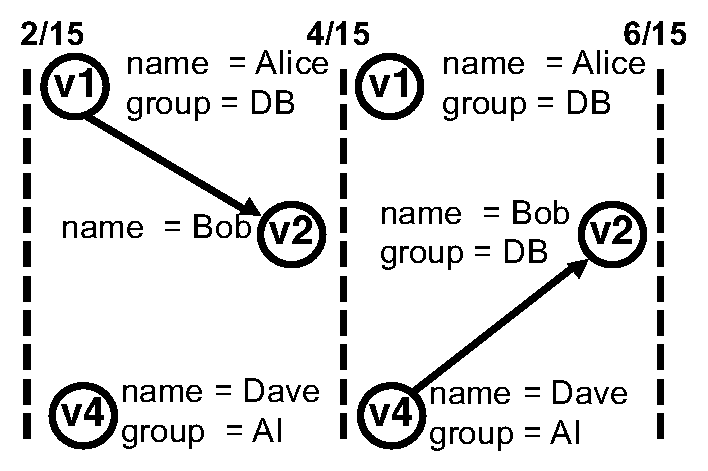
\includegraphics[width=1.35in]{figs/T2_graphs.pdf}
\caption{T2.}
\vspace{-0.2cm}
\label{fig:tg_t2}
\end{minipage}
\begin{minipage}{2in}
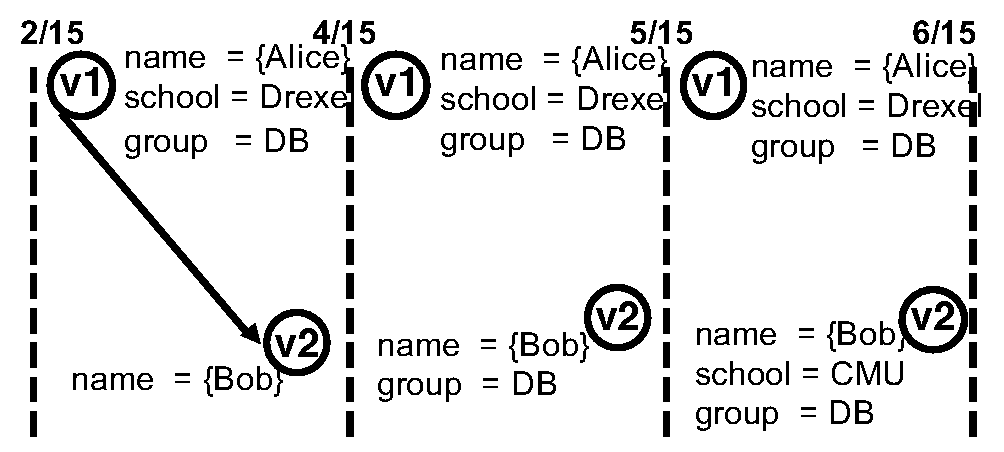
\includegraphics[width=2in]{figs/T1_inter_T2.pdf}
\caption{$T1 \cap^T T2$.}
\vspace{-0.2cm}
\label{fig:tg_inter}
\end{minipage}
\begin{minipage}{3.8in}
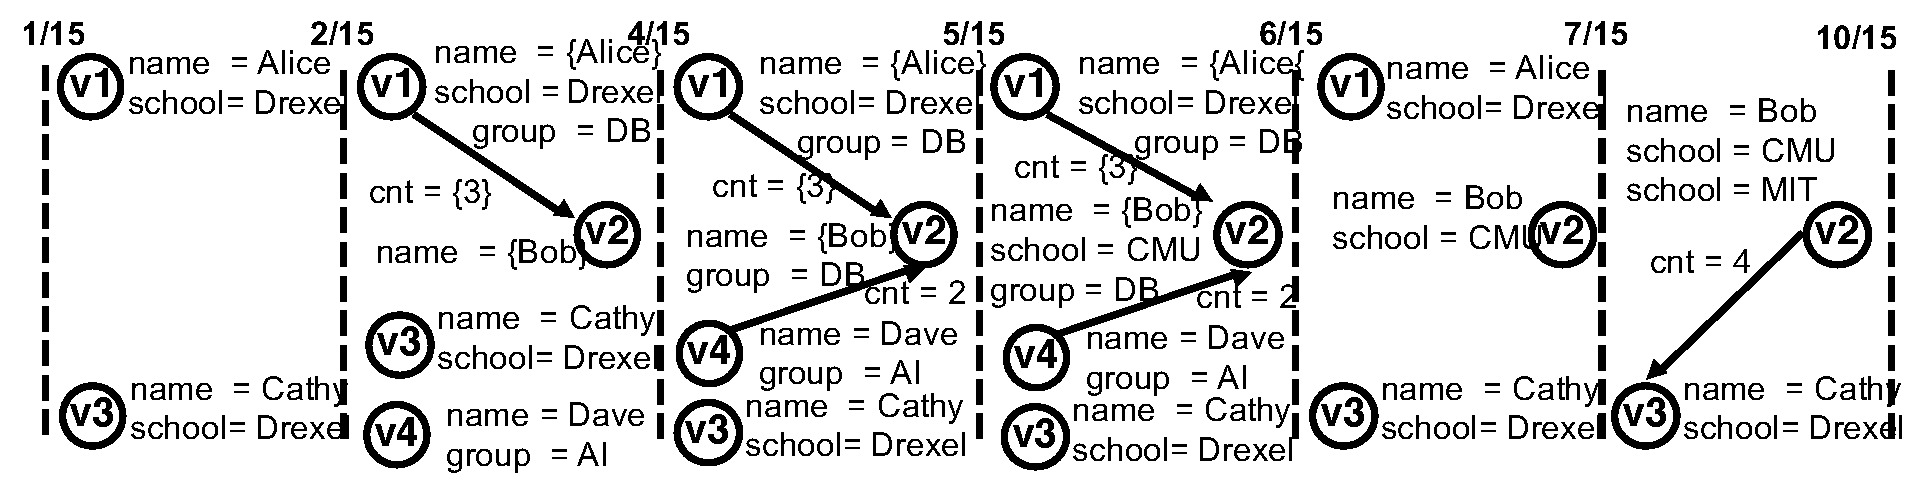
\includegraphics[width=3.8in]{figs/T1_union_T2.pdf}
\caption{$T1 \cup^T T2.$}
\vspace{-0.2cm}
\label{fig:tg_union}
\end{minipage}
\caption{Temporal set operators.}
\label{fig:intersect}
\vspace{-0.2cm}
\end{figure*}

Figure~\ref{fig:intersect} illustrates temporal intersection of \tg
T2, shown in Figure~\ref{fig:tg_t2}, with T1 in our running example,
with a set resolve function for all properties.  Period $[2/15, 4/15)$
  is computed as a result of the join of $[2/15, 5/15)$ in T1 and
    [$2/15, 4/15)$ in T2.  Only the vertices and edges present in both
      \tgs are produced, thus eliminating $v_3$ and $v_4$.  Notice the
      result of attribute set resolve function.
      Figure~\ref{fig:tg_union} is similar to
      Figure~\ref{fig:intersect} but using union instead of
      intersection.  According to the definition of temporal set
      union, periods are split to coincide so that we have 6 total
      periods instead of 5.

Intersection, union, and difference may uncoalesce.  Intersection and
difference require FK enforcement for \tav and \tae, while union does
not.

%\subsection{Temporal graph union}
%\label{sec:algebra:outerjoin}

\eat{
The binary temporal graph union operation $\trga \cup \trgb$ computes
a temporal full outer join~\cite{Gao2005} of \trga and \trgb on the
predicate $\trga.p \cap \trgb.p $. For tuples $(g_1, p_1) \in \trga$
and $(g_2, p_2) \in \trgb$ for which $p_1 \cap p_2 \neq \emptyset$, we
compute $(g_1 \cup g_2, p_1 \cap p_2)$.  The result of $g_1 \cup g_2$
is computed by taking a {\em union} of the sets of vertices and of
edges of the graphs~\cite{GraphTheory}.  For each vertex and edge in
the result, we compute a {\em union} of their bags of properties.
Tuples from \trga (resp. \trgb) for which there does not exist a tuple
in \trgb (resp. \trga) for part or all of the validity period are
included in the result of the full outer join. 
}

\eat{
 $\trg_1 \cup \trg_2 = \{ (g, p) | (g_1, p_1) \in \trg_1 \wedge (g_2,
p_2) \in \trg_2 \wedge ((g = g_1 \cup g_2 \wedge p = p_1 \cap p_2
\wedge p_1 \cap p_2 \neq \emptyset) \vee (g = g_1 \wedge p = p_1 - p_2
\wedge \nexists p \in \trg_2 = p_1 - p_2) \vee (g = g_2 \wedge p = p_2
- p_1 \wedge \nexists p \in \trg_1 = p_2 - p_1))\}$.  Similar to
temporal intersection, temporal union is essentially an outer
theta-join of $\trg_1$ and $\trg_2$ with a $p_1 \cap p_2$ predicate.
We use the standard graph union definition based on set theory, which
computes unions of the vertex and edge sets from the two
operands~\cite{GraphTheory}.}

\eat{
Algorithm~\ref{alg:union} presents the evaluation of $\tvea \cup
\tveb$.  We compute temporal outer joins over the corresponding \tv,
\te, \tav and \tae.
}

\eat{\begin{algorithm}[t]
\caption{Temporal graph union in \tve.}
\begin{algorithmic}[1]
\REQUIRE $\tvea, \tveb$.\\
\STATE $\tv' = \tv_1 \fullouterjoin^T_v \tv_2$\\
\STATE $\te' = \te_1 \fullouterjoin^T_{v1,v2} \te_2$\\
\STATE $\tav' = \cl (\pi_{v,p,\tav_1.a \cup \tav_2.a}\tav_1 \fullouterjoin^T_v \tav_2)$\\
\STATE $\tae' = \cl (\pi_{v_1,v_2,p,\tae_1.a \cup \tae_2.a}\tae_1 \fullouterjoin^T_{v1,v2} \tae_2)$\\
\RETURN new $\tve (\tv';\te';\tav';\tae')$\\
\end{algorithmic}
\label{alg:union}
\end{algorithm}
}

%\subsection{Temporal graph difference}
%\label{sec:algebra:diff}

\eat{
The binary temporal graph difference operation $\trga \setminus \trgb$
computes a temporal left outer join~\cite{Gao2005} of \trga and \trgb
on the predicate $\trga.p \cap \trgb.p$.  For tuples $(g_1, p_1) \in
\trga$ and $(g_2, p_2) \in \trgb$ for which $p_1 \cap p2 \neq
\emptyset$, we compute $(g_1 \setminus g_2, p_1 \cap p_2)$.  The
result of $g_1 \setminus g_2$ is computed by taking a {\em set
  difference} of the sets of vertices and of edges of the graphs.  For
each vertex and edge in the result, we compute a {\em union} of their
bags of properties.  Tuples in \trga for which there does not exist a
tuple in \trgb for part or all of the validity period are included in
the result of the left outer join.
}
\eat{
Algorithm~\ref{alg:diff} presents the evaluation of $\tvea \setminus
\tveb$.  We compute temporal left outer joins over the corresponding
\tv and \te (lines 1,2).  We then compute $\tav'$ and $\tae'$ with
temporal outer joins of the corresponding relations (lines 3, 4).
Finally, we enforce foreign key constraints on $\te'$, $\tav'$, and
$\tae'$ (lines 5, 6).
}

\eat{\begin{algorithm}[b]
\caption{Temporal graph difference in \tve.}
\begin{algorithmic}[1]
\REQUIRE $\tvea, \tveb$.\\
\STATE $\tv' = \tv_1 \leftouterjoin^T_v \tv_2$\\ 
\STATE $\te' = \te_1 \leftouterjoin^T_{v_1,v_2} \te_2$\\ 
\STATE $\tav' = \cl (\pi_{v,p,\tav_1.a \cup \tav_2.a}\tav_1 \fullouterjoin^T_v \tav_2)$\\
\STATE $\tae' = \cl (\pi_{v_1,v_2,p,\tae_1.a \cup \tae_2.a}\tae_1 \fullouterjoin^T_{v_1,v_2} \tae_2)$\\
\STATE enforce foreign keys on $\tav'$ w.r.t. $\tv'$\\ 
\STATE enforce foreign keys on $\tae'$ w.r.t. $\te'$\\ 
\RETURN new $\tve (\tv';\te';\tav';\tae')$\\
\end{algorithmic}
\label{alg:diff}
\end{algorithm}
}

\subsection{Aggregation}
\label{sec:algebra:agg}

Aggregation is a common graph operation that can be used to compute
simple properties such as in-degrees of nodes or more complex ones
such as a set of places that all close friends have visited in the
past year.  Aggregation is denoted $\gamma_{C_V,C_E,A_V}$, where $C_V$
is a predicate over the source and destination nodes of the edge,
$C_E$ is a predicate over the edge itself, and $A_V$ is an aggregation
function.  The result is a new graph $\gamma_{C_V,C_E,A_V} (\tve) =
\tve \cup^T \{ \tv, \te, \tav', \tae \}$, where $\tav' =
A_V(\sigma_{C_V,C_E} (\tae \fullouterjoin^T_{vid1=vid} \tav
\fullouterjoin^T_{vid2=vid} \tav))$.  The $C_V$ and $C_E$ predicates
may include temporal clauses.  We show in Section~\ref{sec:sys:impl}
how this is supported through an expansion operation if implemented
directly over the \tve representation.  The temporal union is used to
add the new attribute to the output since it may have different
periods of validity.  For example, while each node in \tg may remain
unchanged for the whole duration, aggregating node degrees would
result in an attribute value for each period of topology change.

Aggregation does not uncoalesce and does not require FK enforcement.

\subsection{Node creation}
\label{sec:algebra:create}

We argued in the introduction that it is interesting and insightful to
analyze an evolving graph at different levels of granularity.  For
example, the user may want to aggregate multiple consecutive
representative graphs into a single representative graph, coarsening
the granularity, or to predefine temporal resolution and look at the
graph at that scale, irrespective of whether this resolution happens
to be finer or coarse than the natural evolution rate of the graph.
For this, we introduce a node creation operator which is similar to
the {\em moving window temporal aggregation} in temporal relational
algebra.  Our approach is inspired by stream aggregation work
of~\cite{Li2005}, adopted to graphs, and by generalized quantifiers
of~\cite{Hsu1995}.

Node creation is denoted $_{G_V}\vartheta_{W,Q_V,Q_E,A_V,A_E}
(\ttt)$,\\ where $G_V$ are the grouping attributes, $W$ is the window
specification, $Q_V$ and $Q_E$ are vertex and edge quantifiers, and
$A_V$ and $A_E$ are the optional aggregation functions.  It produces a
consolidated evolving graph with specific temporal granularity.

{\em Grouping attributes} $G_V$ are vertex properties by which
vertices are grouped into new entities, similar to \insql{GROUP BY}
clause in SQL.  Since node creation requires new identifiers, the
combination of the grouping properties can be used in a mechanism
equivalent to a Skolem function.  The simplest, default grouping
attribute is the $vid$ of the vertex.

{\em Window specification} $W$ is of the form
$n~\{unit|\insql{changes}\}$, where $n$ is an integer, and $unit$ is a
time unit, e.g., $10~min$, $3~years$, or any multiple of the usual
time units.  Window specification of the form $n~\insql{changes}$
defines the window in terms of change over \trg.\eat{ (which may be
  computed from the \tve representation, see
  Section~\ref{sec:model:switch}).}  For example,
$W=3~\insql{changes}$ will aggregate sequences of 3 representative
graphs into 1.  Window boundaries are computed left-to-right, i.e.,
from least to most recent.  The right-most window may correspond to
fewer than $n$ representative graphs from the input.
%
Our window specification by change is similar to slide-by-row window
in stream aggregation~\cite{Li2005}.  Note that, because \tg algebra
is compositional, we do not support node creation with
overlapping windows, because it does not produce a valid \tg.  To see
why this is so, consider applying a sliding window of 3 months range
with 1 month slide to graph \insql{T} in Figure~\ref{fig:tg_rg}.  We
would produce the following set $(g_1, [1/15, 4/15)), (g_2, [4/15,
    7/15)), (g_3, [7/15, 10/15))$, which clearly violates the
      temporally coalesced requirement in
      definition~\ref{tg_abstract}.  

Similar to~\cite{Li2005} we support creation simultaneously by time
and by non-temporal attributes (e.g., vertex properties).  If the
window specification is one change, then the operation devolves into
pure structural reduce or node creation, as classified by
Wood~\cite{Wood2012}.  If the grouping attribute is the vertex $vid$,
then the operation is purely temporal, with no structural aspect.

{\em Quantifiers} $Q_V$ and $Q_E$ are of the form \{ \insql{all} |
\insql{most} | \insql{at least} $n$ | \insql{exists} \}, where $n$ is
a decimal representing the percentage of the time during which an
entity (vertex or edge) existed, relative to the duration of the
window. These are useful for producing different kinds of
representative graphs.  For example, to produce representative graphs
with only strong connections over a volatile evolving graph, we may
want to only include vertices that span the entire time window
($Q_V=\insql{all}$), and edges that span a large portion of the window
($Q_E=\insql{most}$).
 
The optional {\em aggregation functions} $A_V$ and $A_E$ compute new
values for vertex and edge properties representative of
the whole window, e.g., $A_V=\insql{any}(name), \insql{last}(school)$
and $A_E=\insql{sum}(cnt)$.
%
 
Key-value pairs for vertex and edge properties for which no
aggregation functions are specified, are collected into a bag
corresponding to the entity in the result.  These can be subsequently
transformed with $map^T$ (Section~\ref{sec:algebra:project}).

\eat{ 
Temporal aggregation over \tve follows the outline of
Algorithm~\ref{alg:op}, but requires an additional step, and is
revisited in Algorithm~\ref{alg:agg_ve}.
%
}

We compute group periods based on window specification.  Next, as part
of $_{G_V}\vartheta_{P,Q_V}(\tv)$ computation, we assign each tuple from
\tv to a period (this requires splitting), group vertices by $G_V$ and
evaluate $Q_V$ on each group.  Only groups for which $Q_V$ evaluates
to true are retained.  Edges are processed similarly by
$_{G_V}\vartheta_{P,Q_E}(\te)$.  Note that when $G_V$ is anything besides
$vid$, we need edge triplets in order to compute new source and
destination ids of each edge.  As with aggregation above, edge
triplets can be computed through a three-way temporal outerjoin of
\tae with \tav.  $_{G_V}\vartheta_{P,A_V}(\tav)$ and
$_{G_V}\vartheta_{P,A_E}(\tae)$, respectively, are a result of computing
a group for each vertex or edge within the period, and applying the
aggregate functions over each group.

\eat{
Node creation over \trg is computed by first calculating time periods
from $W$ and \trg, and then reducing and combining the representative
graphs directly.
}

\eat{\begin{algorithm}[t!]
\caption{Node creation in \tve.}
\begin{algorithmic}[1]
\REQUIRE \tve (\tv;\te;\tav;\tae), window specification $W$, vertex
quantifier $Q_V$, edge quantifier $Q_E$, vertex aggregate function
$A_V$, vertex aggregate function $A_E$.\\
\STATE $P = \textsf{computePeriods}(W, \tv, \te, \tav, \tae)$\\
\STATE  $\tv' = \cl (_{G_V}\vartheta_{P,Q_V}(\tv))$\\
\STATE  $\te' = \cl (_{G_V}\vartheta_{P,Q_E}(\te))$\\
\STATE  $\tav' = \cl (_{G_V}\vartheta_{P,A_V}(\tav))$\\
\STATE  $\tae' = \cl (_{G_V}\vartheta_{P,A_E}(\tae))$\\
\STATE  follow steps 5-7 of Algorithm~\ref{alg:op}\\
%\STATE  enforce foreign keys on $\te'$ w.r.t. $\tv'$\\
%\STATE  enforce foreign keys on $\tav'$ w.r.t. $\tv'$\\
%\STATE  enforce foreign keys on $\tae'$ w.r.t. $\te'$\\
\RETURN new $\tve (\tv';\te';\tav';\tae')$\\
\end{algorithmic}
\label{alg:agg_ve}
\end{algorithm}
}

Figure~\ref{fig:tg_agg1} illustrates node creation by time
($W=3~\textsf{months}$), and Figure~\ref{fig:tg_agg2} --- by change
($W=3~\textsf{changes}$).  Figure~\ref{fig:tg_agg3} illustrates
structural reduce only ($W=1~\textsf{change}$), and
Figure~\ref{fig:tg_agg4} both structural and temporal
($G_V=\textsf{school}, W=3~\textsf{months}$).  All four are applied to
\insql{T1} in our running example, and list the same quantifiers
(\insql{all} for vertices and \insql{exists} for edges) and aggregate
functions (\insql{first} for vertex and edge properties).  $v_2$ is
present in the result in Figure~\ref{fig:tg_agg1} starting at $4/15$
because it did not exist for the entirety of the first window, while
in Figure~\ref{fig:tg_agg2} it is produced starting $6/15$.  In
Figure~\ref{fig:tg_agg3} vertices $v1$ and $v3$ create a single new
vertex $v1$ representing the institution.  A subsequent \insql{map}
operation to produce a new name attribute and a count of people would
produce a more meaningful final result.

\begin{figure*}[t]
%\centering
\begin{subfigure}[b]{0.5\textwidth}
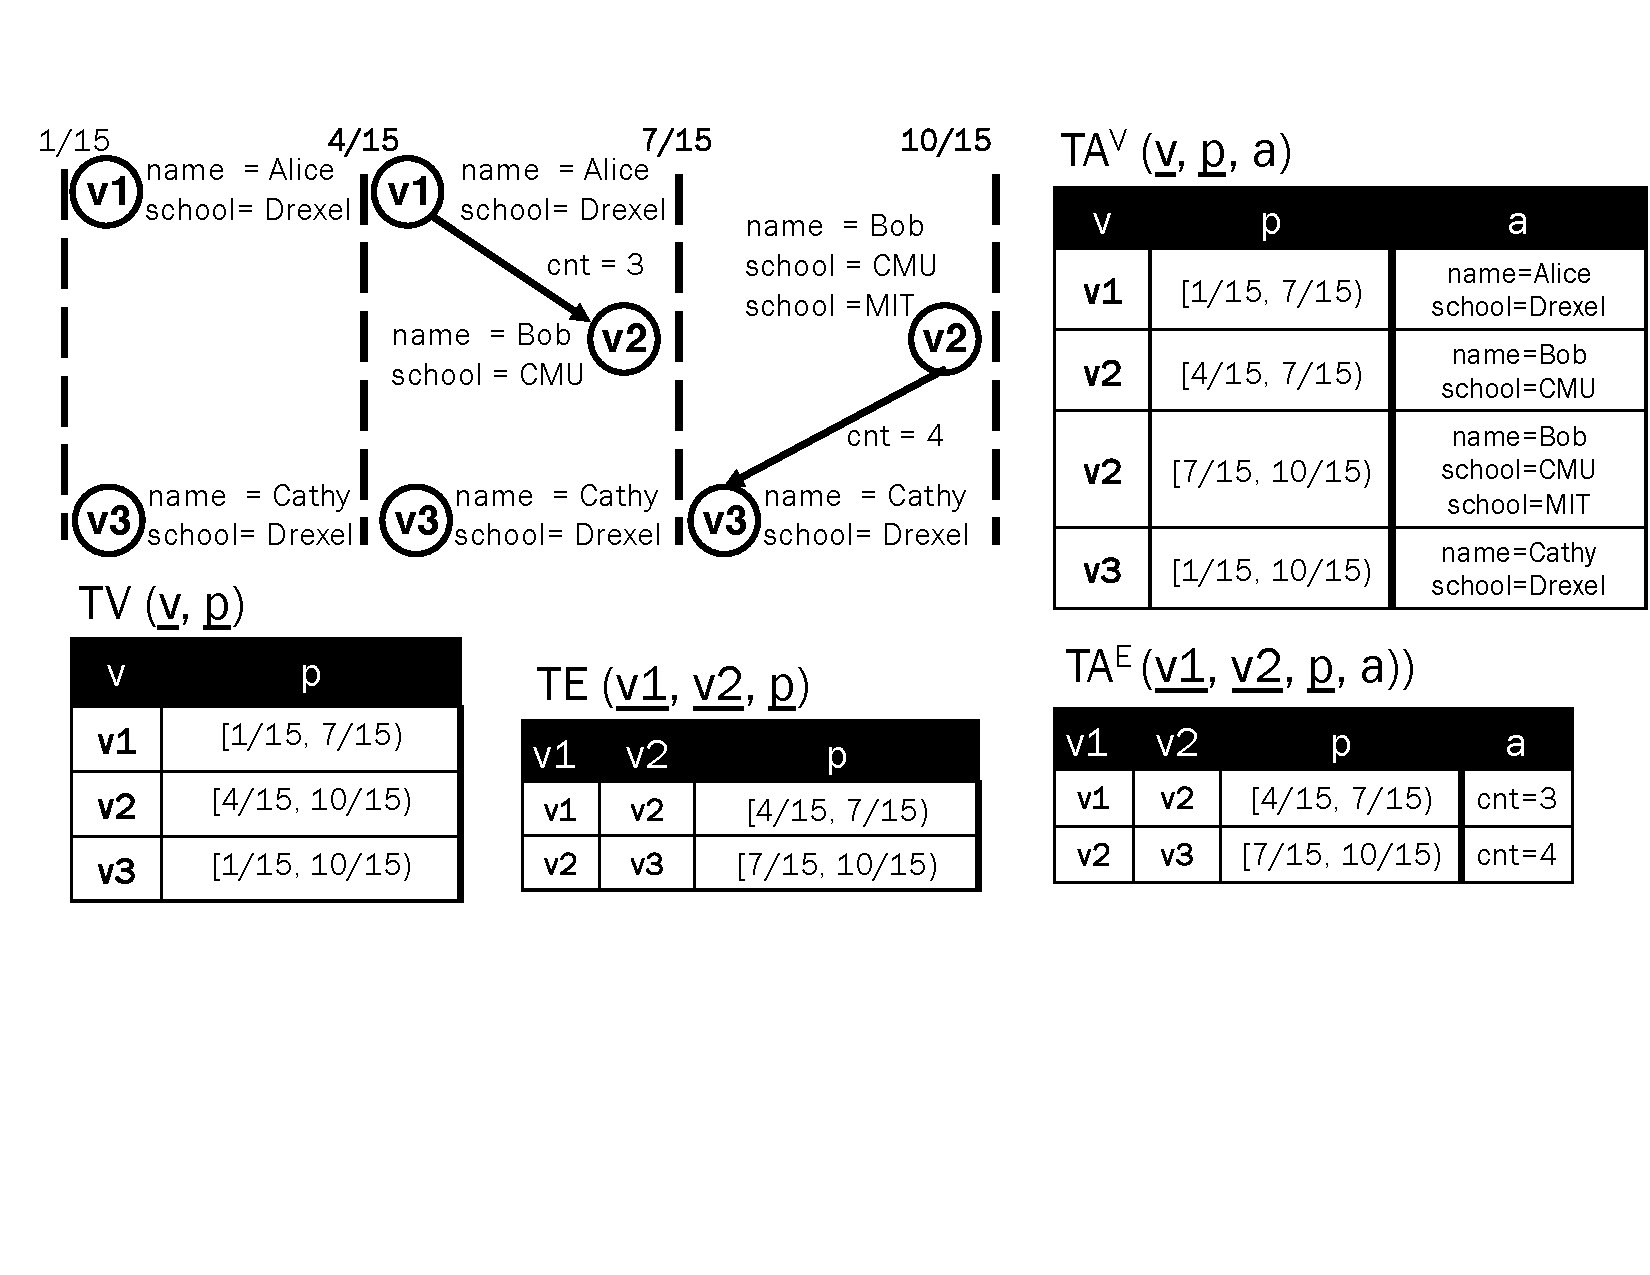
\includegraphics[width=3.5in]{figs/agg1.pdf}
\caption{Node creation from \insql{T1} by time:
  $W=3~\textsf{months}, G_V=\textsf{vid}$.}
\label{fig:tg_agg1}
\end{subfigure}
\begin{subfigure}[b]{0.4\textwidth}
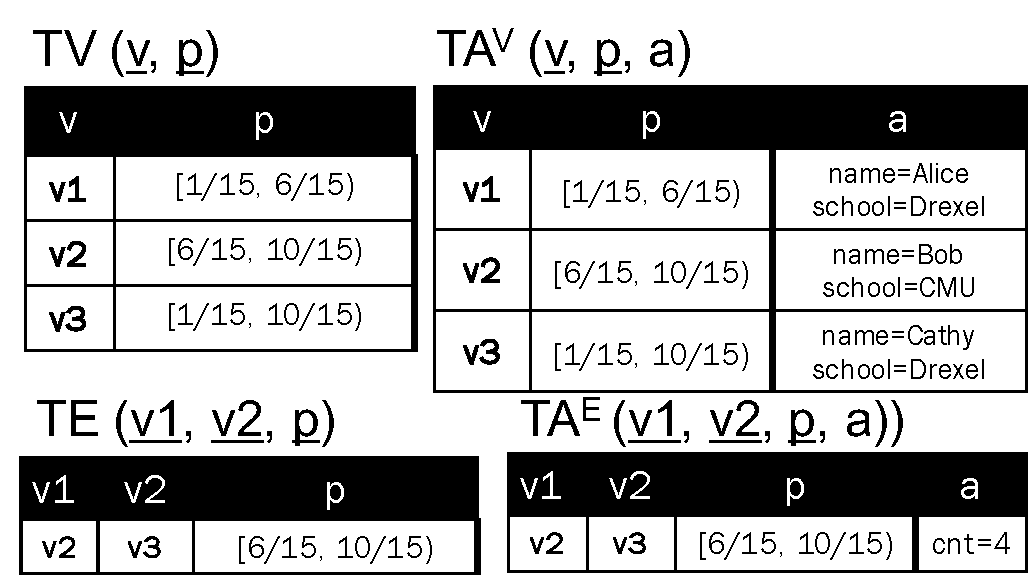
\includegraphics[width=3in]{figs/agg2.pdf}
\caption{Node creation in \insql{T1} by change:
  $W=3~\textsf{changes}, G_V=\textsf{vid}$.}
\label{fig:tg_agg2}
\end{subfigure}
\begin{subfigure}[b]{0.5\textwidth}
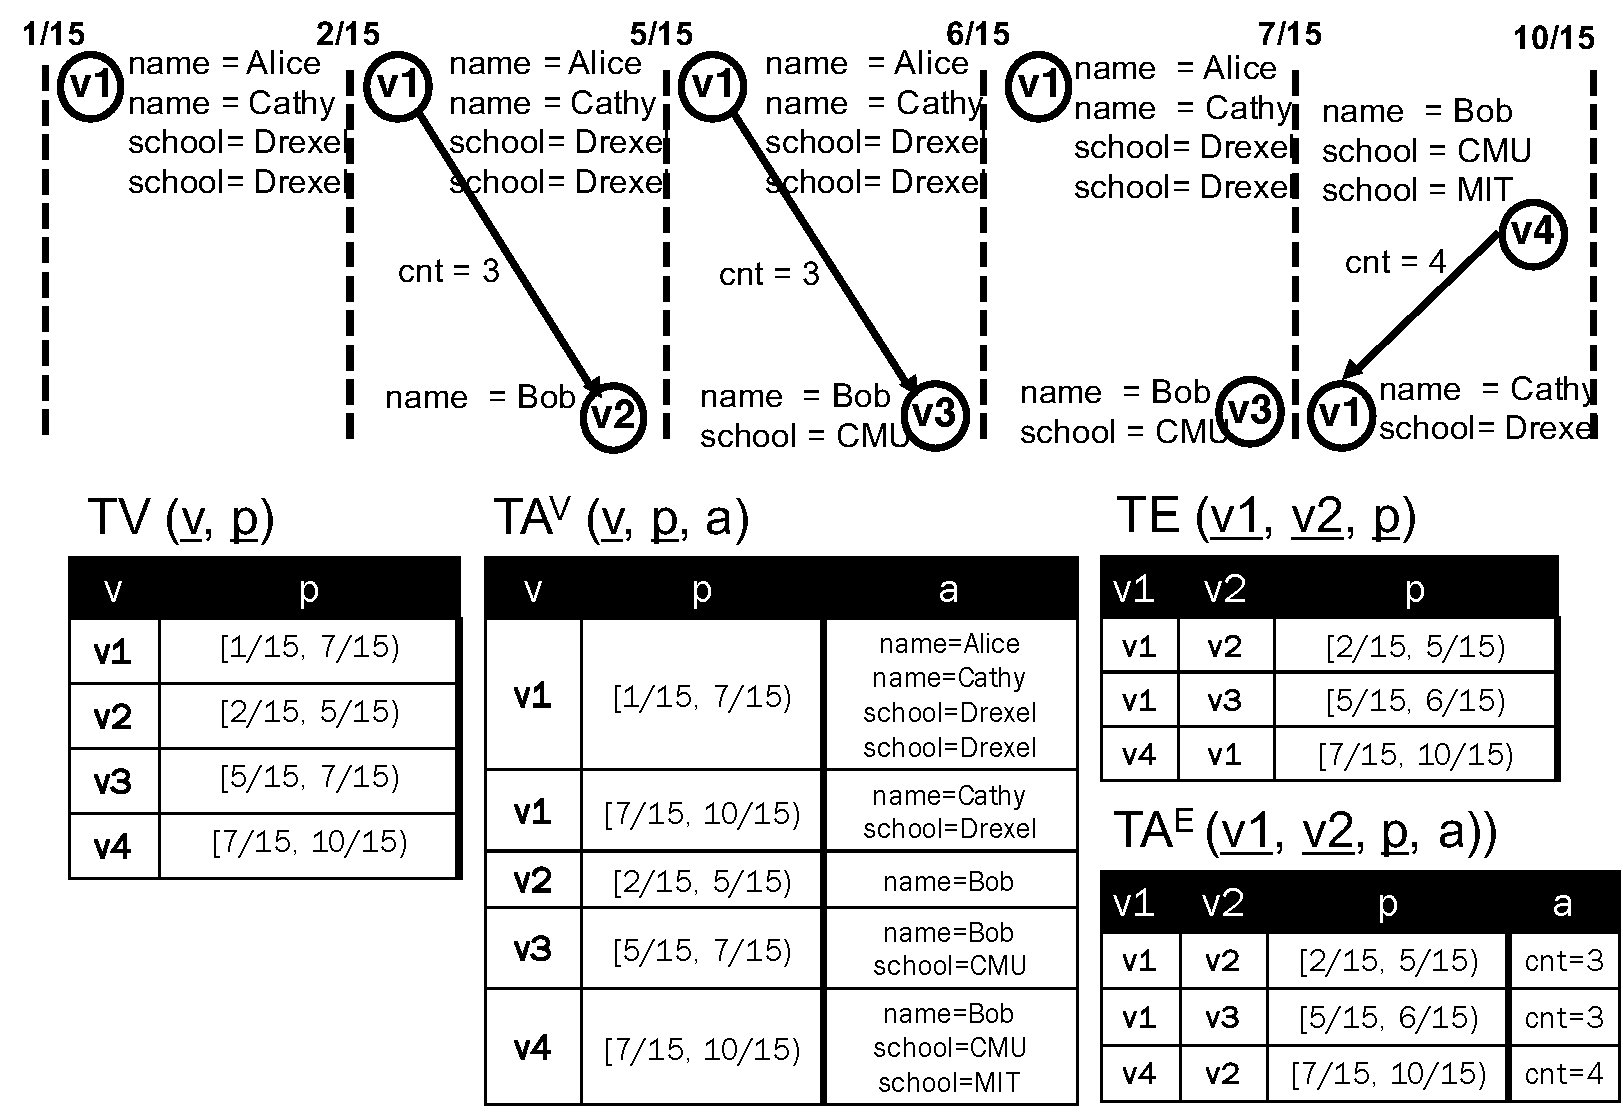
\includegraphics[width=3.5in]{figs/agg3.pdf}
\caption{Node creation in \insql{T1} grouped by attribute:
  $W=1~\textsf{change}, G_V=\textsf{school}$.}
\label{fig:tg_agg3}
\end{subfigure}
\begin{subfigure}[b]{0.4\textwidth}
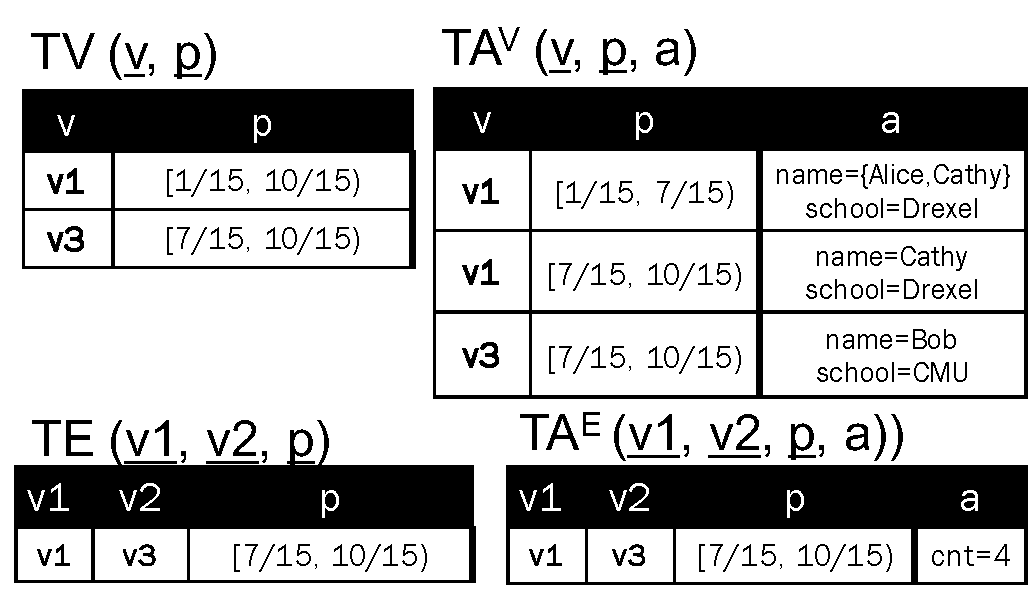
\includegraphics[width=3in]{figs/agg4.pdf}
\caption{Node creation in \insql{T1} by time with grouping:
  $W=3~\textsf{months}, G_V=\textsf{school}$.}
\label{fig:tg_agg4}
\end{subfigure}
\caption[]{Node creation, $Q_V=\insql{all}$, $Q_E=\insql{exists}$,
  $A_V=\insql{first}$, $A_E=\insql{first}.$}
\label{fig:tg_agg}
\vspace{-0.5cm}
\end{figure*}

Node creation may uncoalesce and requires FK enforcement.

\eat{ Our aggregation quantifiers are inspired by generalized
  quantifiers of~\cite{Hsu1995} with n-place delimiters.  $Q(R)$ as a
  Boolean-valued function of a relation''~\cite{Hsu1995}.  A
  quantifier contains an n-place determiner, e.g., ``at least one
  vertex in each window for each group'' is a 2-place determiner
  quantifier.  \tg algebra supports determiners from the set
  $\{at\ least\ one, all, most, at\ least\ n\}$, where $n$ is an
  integer representing a ratio.  $all$ is a usual universal quantifier
  that in standard SQL can be achieved with the use of two \insql{NOT
    EXISTS}.}

\subsection{Transitive closure}
\label{sec:algebra:closure}

TODO


\eat{So far we have defined the operations in our temporal graph
  algebra.  Next we define another class of non-algebraic operations
  on evolving graphs that are nevertheless very useful: analytics.}

\eat{\vera{What I think we are leaving out: difference, structural
  aggregation (new entity creation), graph joins and products (maybe?
  graph joins are weird), more general select (with time in predicate
  and/or path predicates), reverse/transpose.}}
